\section{Ergebnisse}
Die Zusammenfassung der Ergebnisse ist in \autoref{anh:ergebnisse} zu finden und umfasst vier Tabellen. Die Aufteilung in die vier Tabellen geschah entsprechend der Kompressionsverfahren, das bedeutet eine Tabelle enthält die Ergebnisse aller drei Kompressionsraten, aufgeteilt in die drei Datensätze und in die vier Analyseverfahren. Die ersten vier Werte entsprechen richtig positiv, richtig negativ, falsch positiv und falsch negativ, während die letzten beiden Werte für Sensitivität und Präzision stehen (siehe \autoref{sec:auswertung} für Bedeutungen und Abkürzungen). In dem folgenden Abschnitt sind diese Ergebnisse in vier Abbildungen mit jeweils drei Plots der F$_1$"=Maße aufgeteilt. Die Aufteilung geschah auch hier entsprechend der Kompressionsverfahren, das bedeutet in einer Abbildung findet sich ein Plot je Datensatz. Die x"=Achse eines Plots stellt die Kompressionsrate dar und die y"=Achse das F$_1$"=Maß. Die verschiedenfarbigen Linien zeigen die Entwicklung des F$_1$"=Maßes eines Analyseverfahrens, entlang sinkender Kompressionsrate. In zwei Plots sind nur drei Linien zu erkennen, was daran liegt, dass manche Verfahren identische Ergebnisse lieferten und somit sich überlagern. So in \autoref{subfig:f1linnvidia} die Verfahren knn und iForest und in \autoref{subfig:f1fouriernvidia} die Verfahren knn und Ähnlichkeitssuche.

In einem ersten Blick fällt auf, dass die Analyseverfahren zu einem großen Teil gut abschnitten. Dass bedeutet, dass in den meisten Fällen das F$_1$"=Maß über 0,7 lag und somit ein gutes Gleichgewicht zwischen Sensitivität und Präzision herrscht, egal welches Kompressionsverfahren und "=rate. Allerdings gibt es auch äußerst schlechte Ergebnisse, so zum Beispiel in \autoref{subfig:f1polecg}, wo nahezu alle Werte unter 0,5 liegen oder die Random Projection sogar dauerhaft F$_1$"=Maße von 0,0 oder leicht darüber besitzt. Generell fällt auch auf, dass die EKG"=Daten aus dem ECG5000 Datensatz am schlechtesten performen. So sind dort die meisten Werte unter 0,7 und schwanken auch um 0,7, was bedeutet, dass die Verfahren unterschiedlich gut beziehungsweise schlecht abschneiden. Bei den anderen beiden Datensätzen schwanken die Werte hingegen um 0,3, bis auf die Ausnahme von ein paar wenigen Ausreißern.

Schauen wir uns nun die Ergebnisse mit Fokus auf die Kompressionsverfahren an, so liefern die Wavelet"= und lineare Kompression in fast allen Fällen stabile Ergebnisse mit nur geringen Verlusten gegenüber den unkompromierten Daten. Dagegen führen Fourier"= und polynomielle Kompression häufig zu einem deutlichen Leistungsabfall. So sinkt beispielsweise das F$_1$"=Maß beim Datensatz ECG5000 bei Fourier"=Kompression auf Werte unter 0,3, während Wavelet"= und lineare Kompression auf demselben Datensatz weiterhin Werte oberhalb von 0,7 erreichen. Auch interessant ist, dass die Wetterdaten eigentlich konsequent gute Ergebnisse erzielen, jedoch bei der Fourier"=Kompression in \autoref{subfig:f1fourierwetter} die meisten Werte unter 0,8 liegen oder die Random Projection sogar komplett einbricht und ironischerweise bei der niedrigsten Kompressionsrate die besseren Ergebnisse erzielt. Damit wird klar, dass nicht alle Kompressionsverfahren gleichermaßen geeignet sind, um die gewollte Qualität der anschließenden Analyseverfahren zu erhalten.

Auch zwischen den Analyseverfahren treten deutliche Unterschiede auf. So erweist sich die Ähnlichkeitssuche insgesamt als am robustesten gegenüber Kompression. Selbst bei hohen Kompressionsraten bleibt das F$_1$"=Maß stabil. Random Projection hingegen zeigt stärkere Schwankungen und ist insbesondere bei Fourier"=Kompression anfällig für Qualitätsverluste. Das iForest-Verfahren liefert die schwächsten Resultate unter Kompression und bricht in mehreren Fällen deutlich ein, sodass die Erkennungsleistung teilweise nicht mehr brauchbar ist oder zumindest schlechter als die anderen Ausreißererkennungsverfahren.

Zusammenfassend lässt sich festhalten, dass Wavelet"= und lineare Kompression durchgängig gute Resultate erzielen, während Fourier"= und polynomielle Kompression die Ausreißererkennung stark beeinträchtigen. Unter den Analyseverfahren zeigt sich die Ähnlichkeitssuche als am robustesten, wohingegen iForest unter Kompression stark an Qualität verliert.

In den nachfolgenden Tabellen \ref{tbl:laufzeitlin}, \ref{tbl:laufzeitpol}, \ref{tbl:laufzeitfour} und \ref{tbl:laufzeitwav} sind die prozentualen Laufzeiten der Analyseverfahren aufgelistet, also die benötigte Zeit auf den komprimierten Daten im Verhältnis zur Laufzeit auf den Originaldaten. Zu erkennen ist dass, egal welches Verfahren, die Laufzeiten auf den komprimierten Daten kürzer sind als auf den originalen Daten. Vor allem knn profitiert enorm von der Komprimierung, so braucht das Verfahren in manchen Fällen nur noch 3\% der ursprünglichen Zeit. Außerdem ist zu beobachten, dass die Laufzeiten sinken, mit sinkender Kompressionsrate. Ein paar Ausnahmen bei denen das nicht der Fall ist, so z.B. in \autoref{tbl:laufzeitpol} bei ECG5000 und dem Ausreißererkennungsverfahren knn bei dem die Laufzeit für $\rho=0,10$ größer ist als bei $\rho=0,25$, sind auf Messungenauigkeiten zurückzuführen, da die Laufzeiten immer unter 1~s lagen.

In \autoref{fig:alle} sind sechs Plots mit jeweils vier Zeitreihen zu finden. Diese Plots sollen Beispiele von Zeitreihen zeigen, die im komprimierten Zustand nicht mehr erkannt wurden. Dafür ist die nicht mehr erkannte Zeitreihe jeweils rot gefärbt und die drei weiteren grün. Die Grünen sind ebenfalls Ausreißer, und zwar welche mit einem ähnlichen Ausreißer"=Score wie der Ausreißer der nicht mehr erkannt wurde. Erkannt bedeutet hierbei entweder als Ausreißer erkannt oder bei der Ähnlichkeitssuche in \autoref{subfig:abbtwo} als Nachbar erkannt. Die Bildunterschriften enthalten verkürzt die Information in welchem Fall der Ausreißer nicht mehr erkannt wurde. So wird zuerst der Datensatz, dann das Kompressionsverfahren, dann das Analyseverfahren und dann die Kompressionsrate genannt. Ein konkretes Muster, wann ein Ausreißer nicht mehr erkannt wurde, konnten wir nicht entdecken. So lassen sich zwar nachvollziehbare Trends erkennen, jedoch nicht, ab wann ein Ausreißer beziehungsweise Nachbar nicht mehr erkannt wird. Anhand von \autoref{subfig:abbone} und \autoref{subfig:abbtwo} wird deutlich, dass eine Zeitreihe, die den übrigen Zeitreihen stark ähnelt und daher auch bei hoher Kompression eigentlich noch erkennbar sein sollte, nicht mehr detektiert wurde. Gleichzeitig zeigt sich, dass auch weniger ähnliche Zeitreihen bereits bei geringerer Kompression nicht mehr erkannt werden. In \autoref{subfig:abbfive} und \autoref{subfig:abbsix} ist wiederum gegenteiliges zu erkennen, dort ist bei geringer Kompression eine ähnliche Zeitreihe bereits nicht mehr erkannt worden und bei stärkerer Kompression erst eine weit entfernte. Allerdings vergleichen wir hier in den Abbildungen auch verschiedene Analyseverfahren miteinander und das auch noch mit unterschiedlichen Kompressionsverfahren. Insgesamt zeigt sich damit, dass die Kompression die Erkennung von Ausreißern auf komplexe und vom jeweiligen Verfahren abhängige Weise beeinflusst, sodass keine allgemeingültige Grenze für den Informationsverlust angegeben werden kann.

\begin{figure}[htb]
  \subfloat[Wetterdaten]{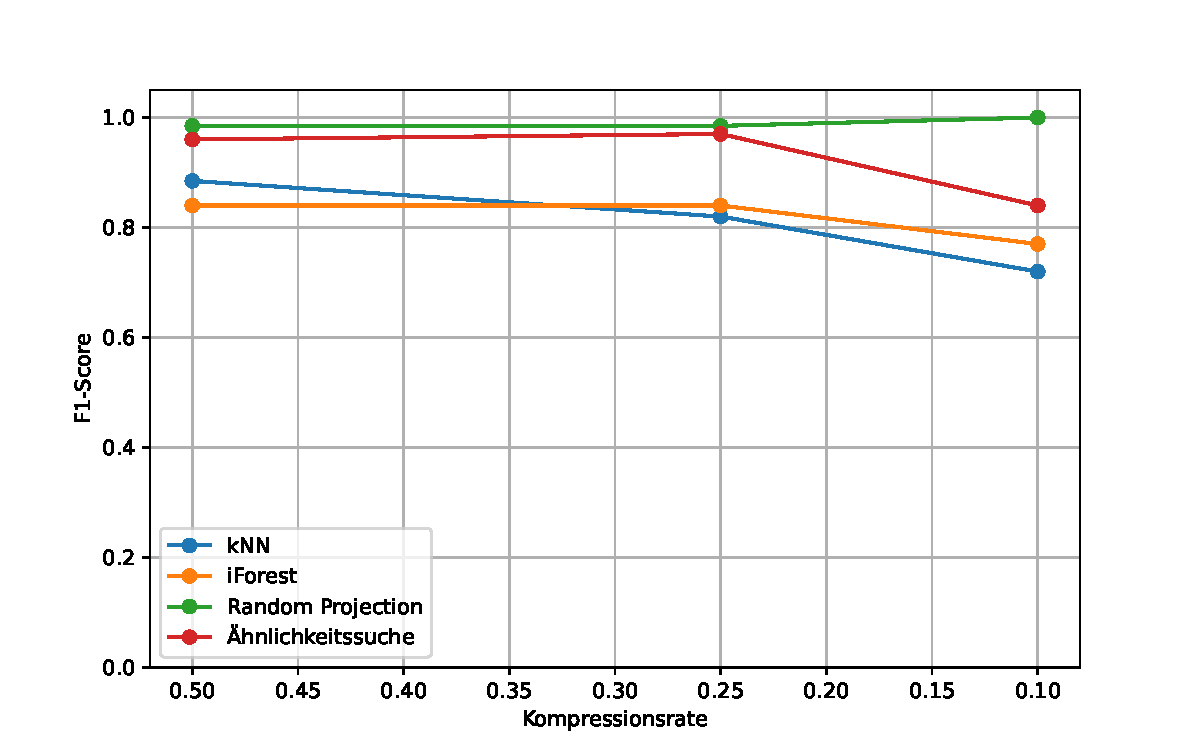
\includegraphics[width=0.49\textwidth]{Graphics/F1LinearWetter.pdf}\label{subfig:f1linwetter}}\hfill
  \subfloat[NVIDIA]{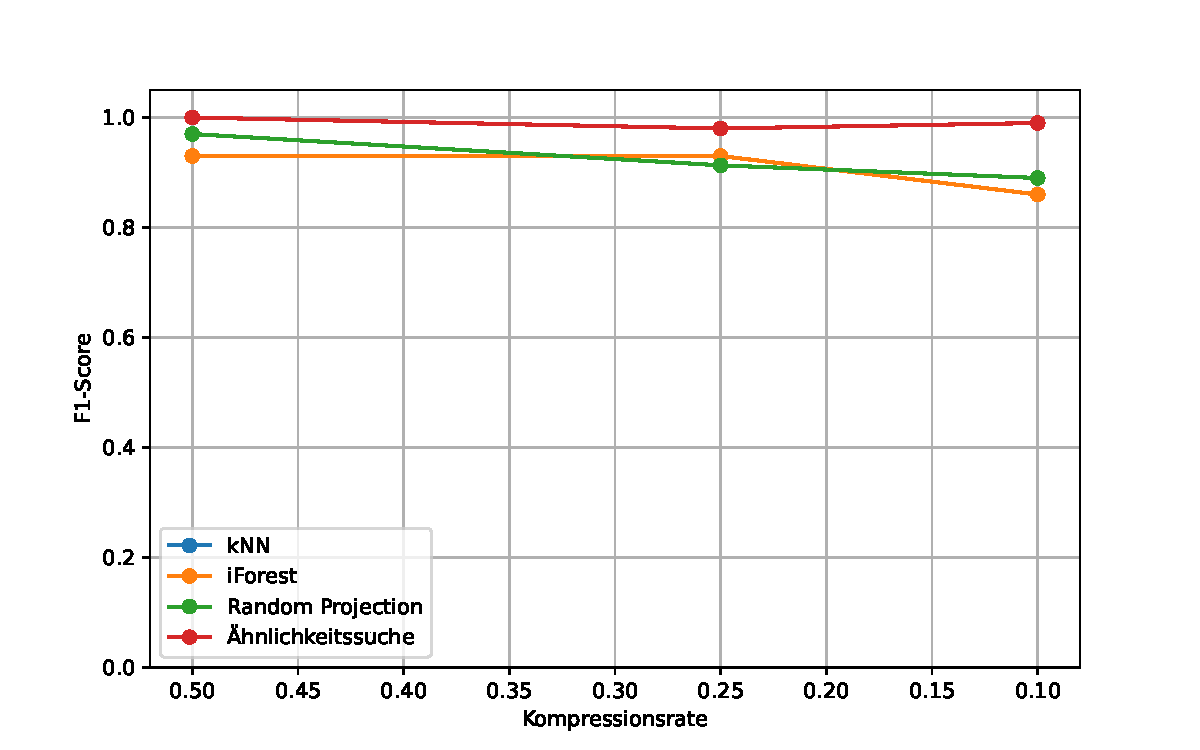
\includegraphics[width=0.49\textwidth]{Graphics/F1LinearNvidia.pdf}\label{subfig:f1linnvidia}}\hfill
  \centering\subfloat[ECG5000]{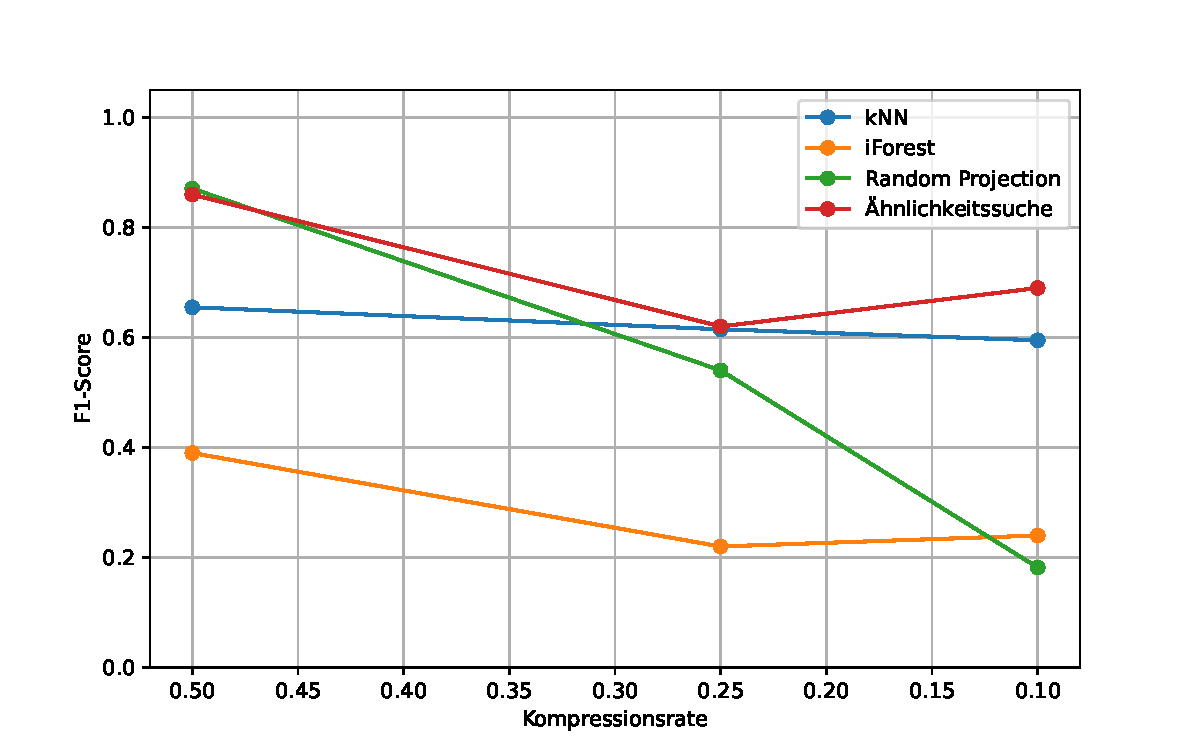
\includegraphics[width=0.49\textwidth]{Graphics/F1LinearECG.pdf}\label{subfig:f1linecg}}
  \caption{F1"=Maße der Analyseverfahren bei linearer Kompression}
  \label{fig:f1LinMaße}
\end{figure}

\begin{figure}[htb]
  \subfloat[Wetterdaten]{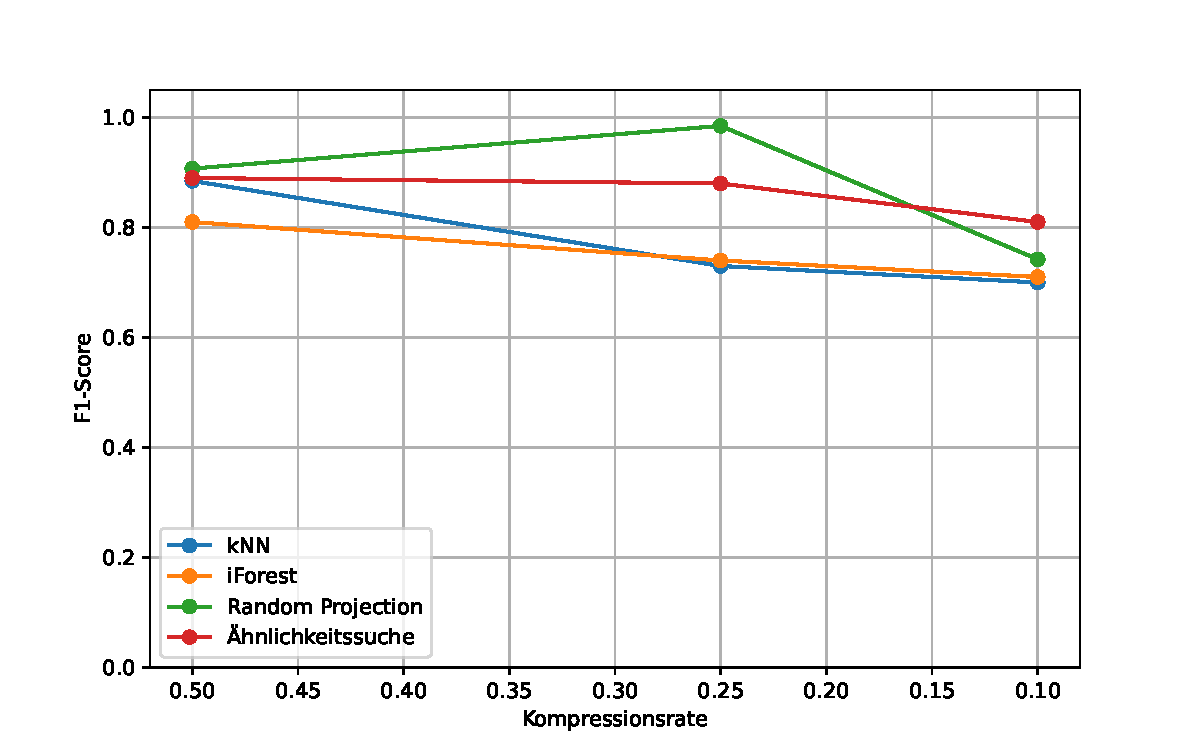
\includegraphics[width=0.49\textwidth]{Graphics/F1PolyWetter.pdf}\label{subfig:f1polwetter}}\hfill
  \subfloat[NVIDIA]{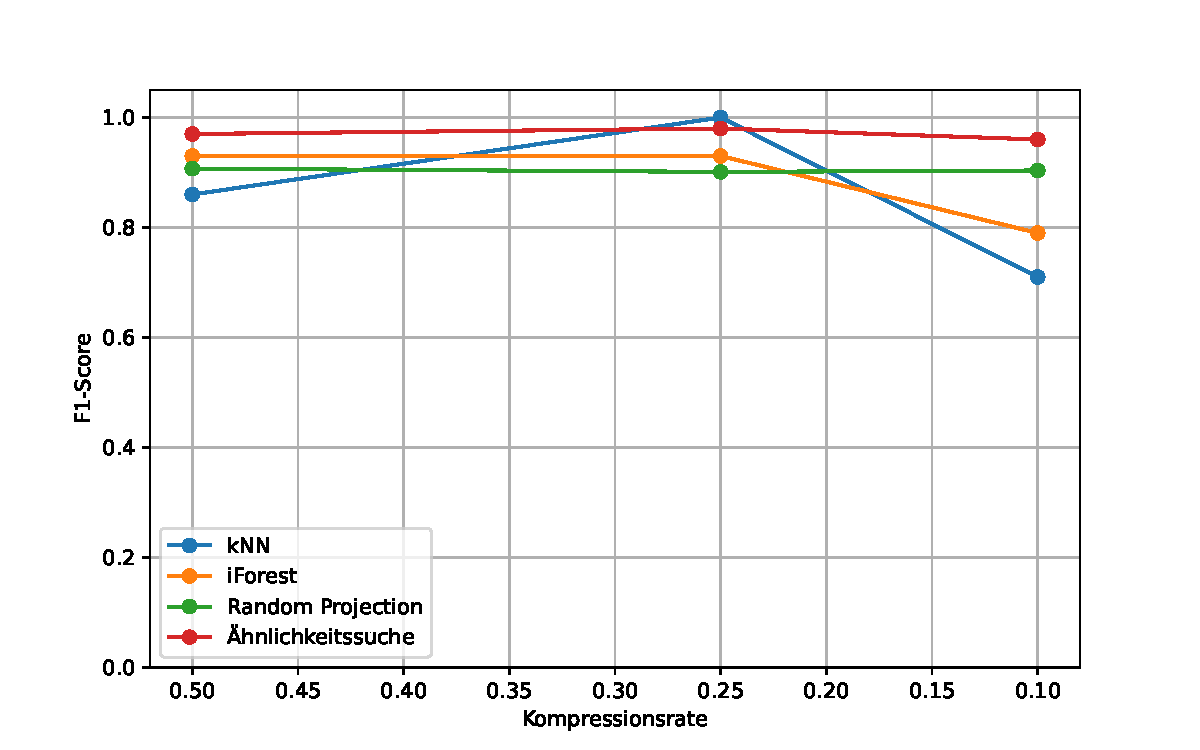
\includegraphics[width=0.49\textwidth]{Graphics/F1PolyNvidia.pdf}\label{subfig:f1polnvidia}}\hfill
  \centering\subfloat[ECG5000]{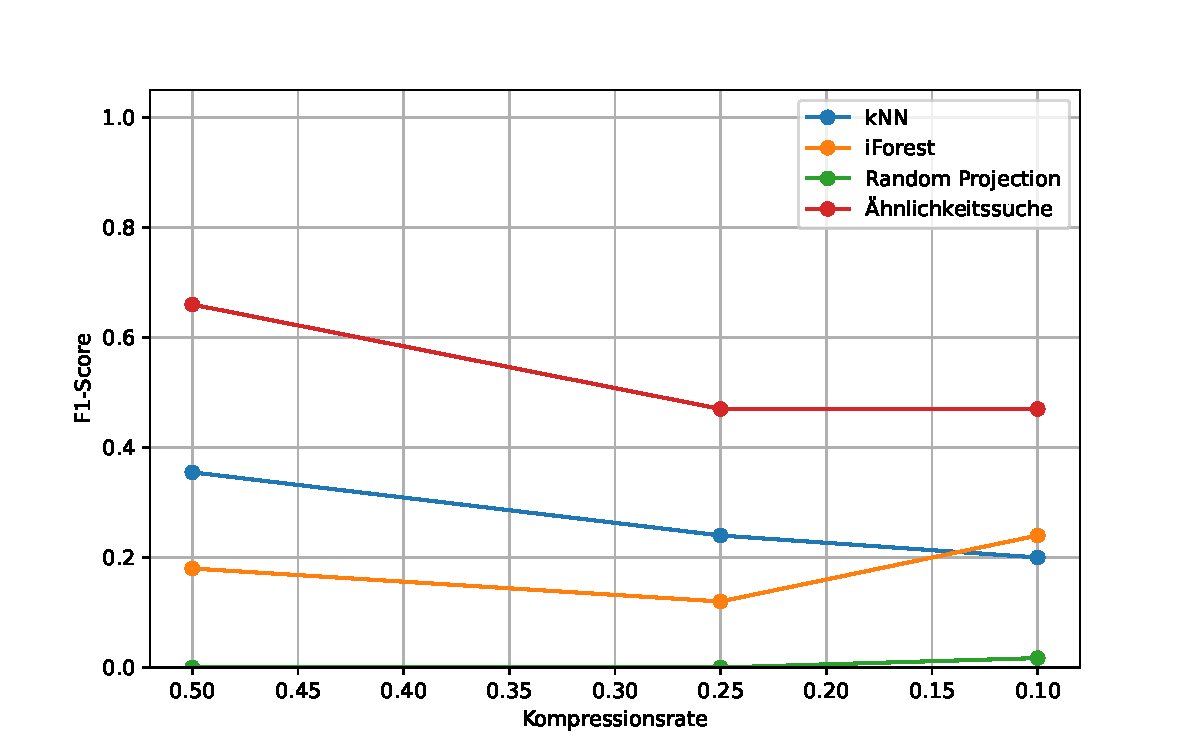
\includegraphics[width=0.49\textwidth]{Graphics/F1PolyECG.pdf}\label{subfig:f1polecg}}
  \caption{F1"=Maße der Analyseverfahren bei polynomieller Kompression}
  \label{fig:f1PolMaße}
\end{figure}

\begin{figure}[htb]
  \subfloat[Wetterdaten]{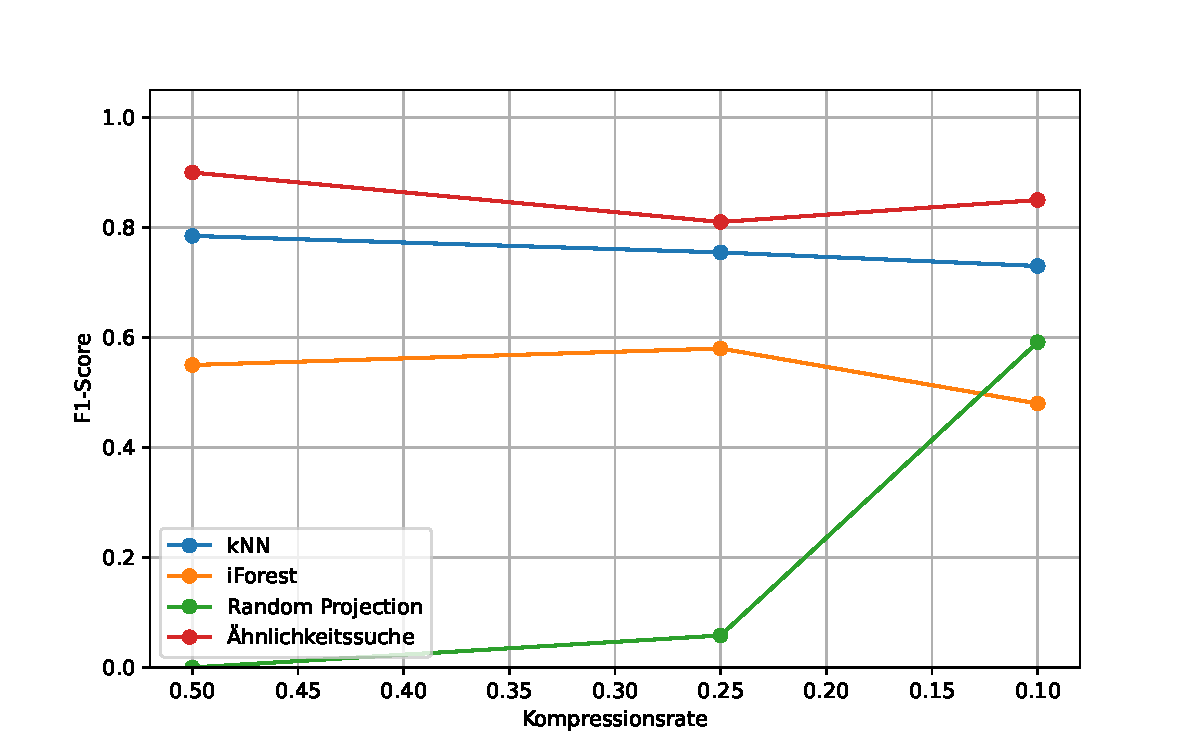
\includegraphics[width=0.49\textwidth]{Graphics/F1FourierWetter.pdf}\label{subfig:f1fourierwetter}}\hfill
  \subfloat[NVIDIA]{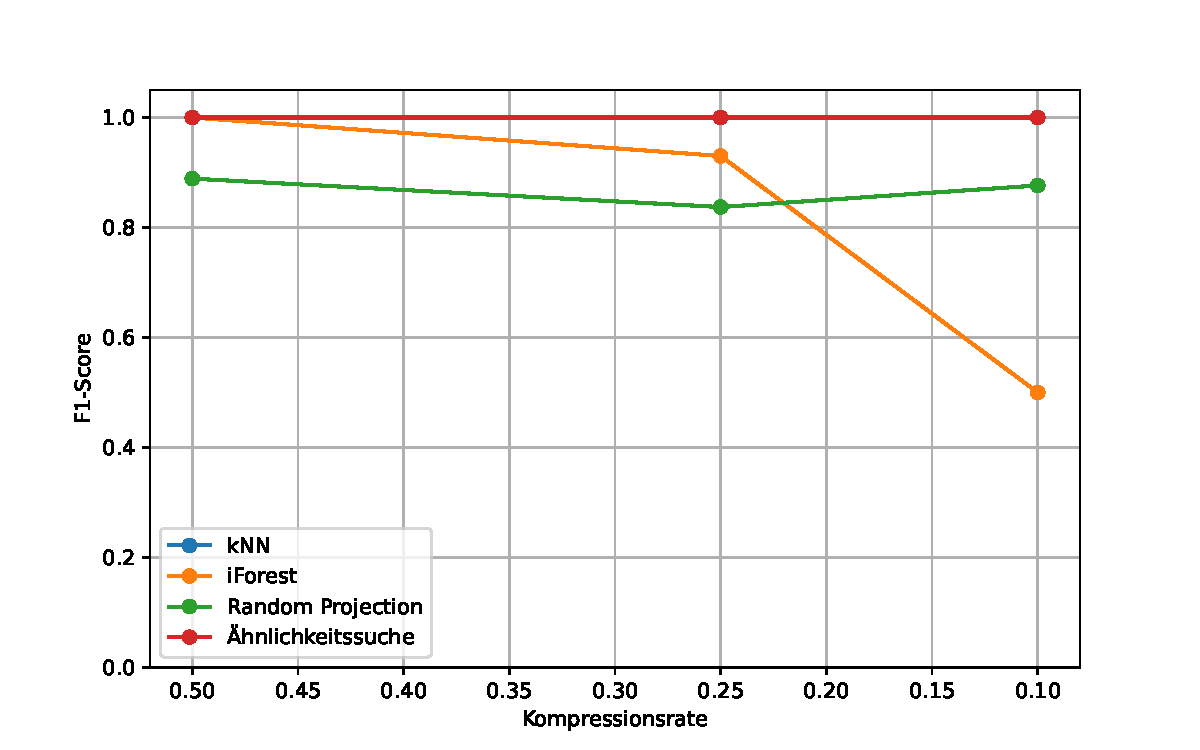
\includegraphics[width=0.49\textwidth]{Graphics/F1FourierNvidia.pdf}\label{subfig:f1fouriernvidia}}\hfill
  \centering\subfloat[ECG5000]{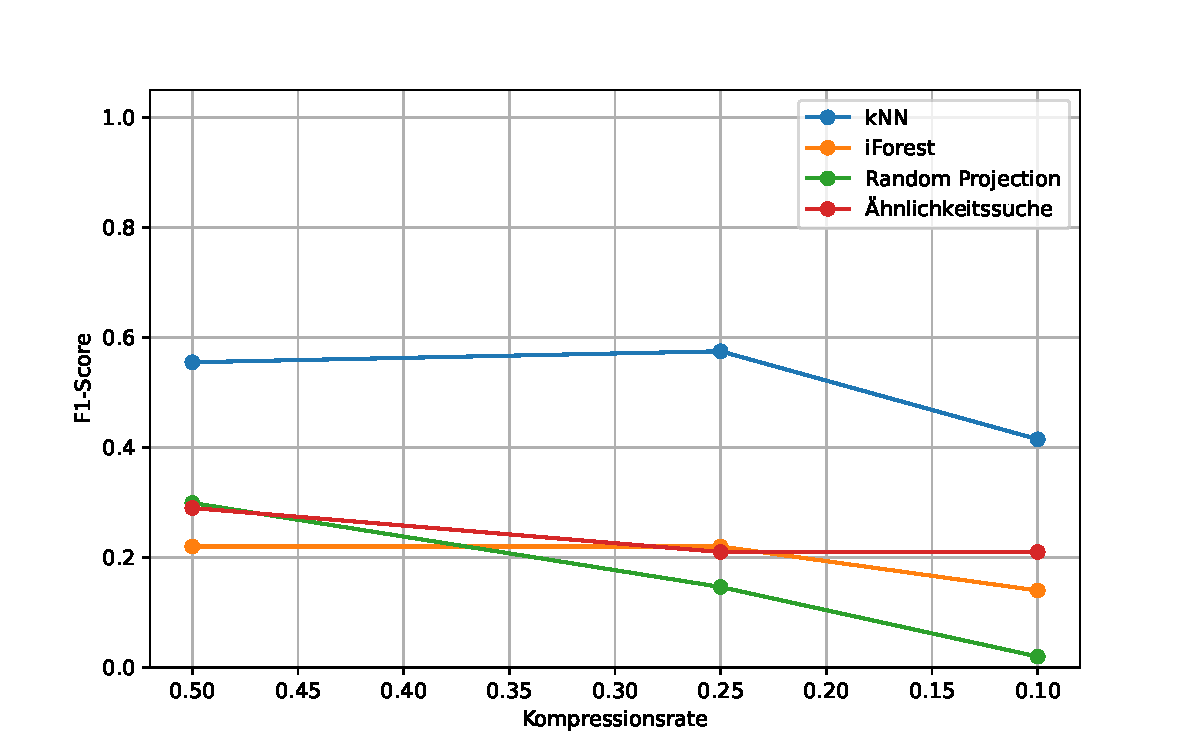
\includegraphics[width=0.49\textwidth]{Graphics/F1FourierECG.pdf}\label{subfig:f1fourierecg}}
  \caption{F1"=Maße der Analyseverfahren bei Fourier"=Kompression}
  \label{fig:f1FourMaße}
\end{figure}

\begin{figure}[htb]
  \subfloat[Wetterdaten]{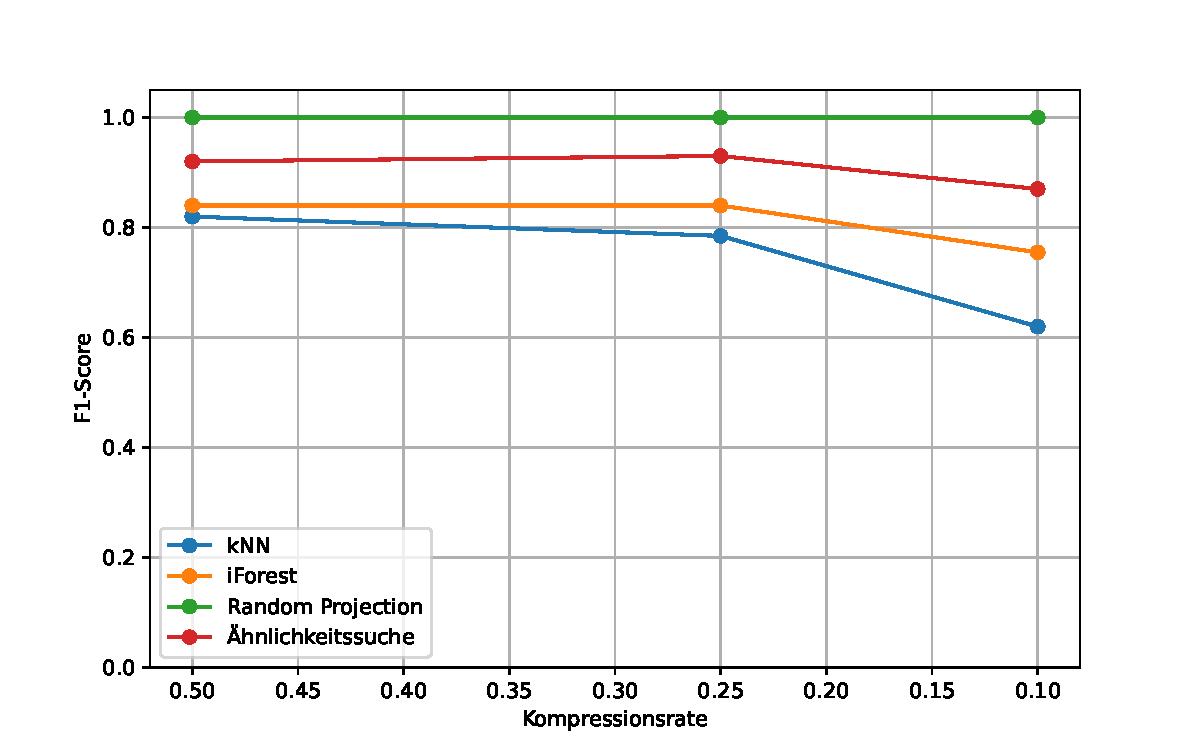
\includegraphics[width=0.49\textwidth]{Graphics/F1WaveletWetter.pdf}\label{subfig:f1waveletwetter}}\hfill
  \subfloat[NVIDIA]{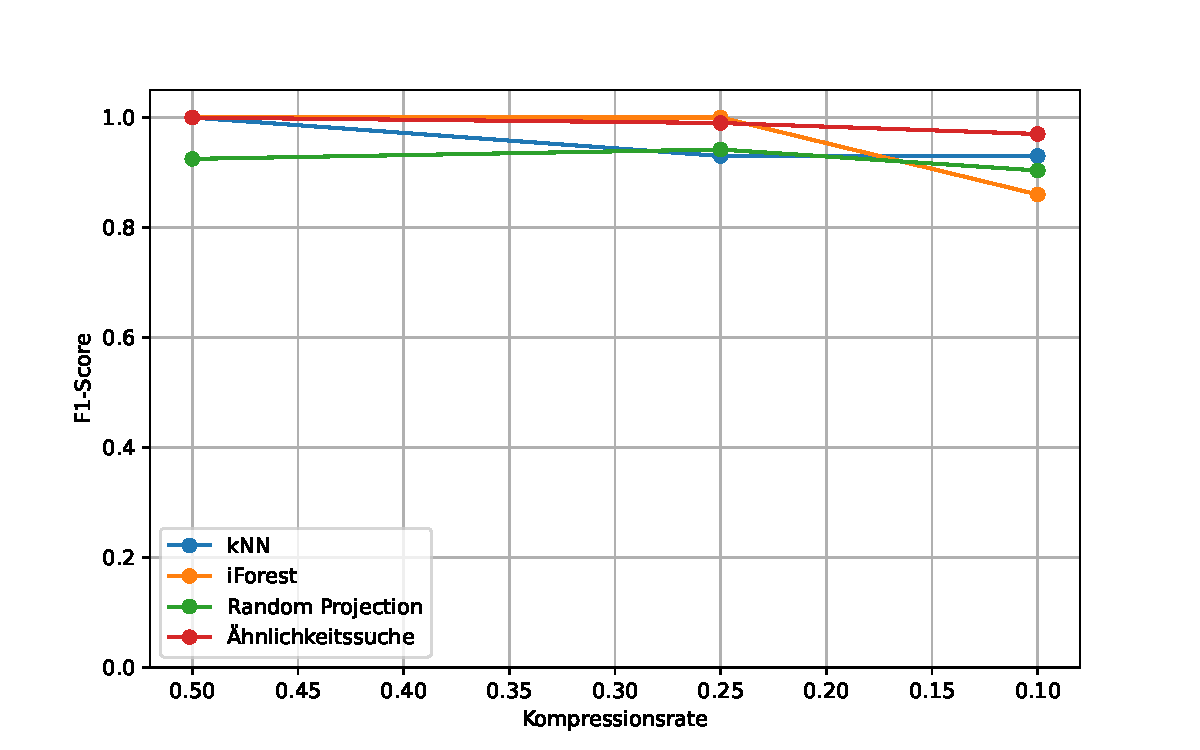
\includegraphics[width=0.49\textwidth]{Graphics/F1WaveletNvidia.pdf}\label{subfig:f1waveletnvidia}}\hfill
  \centering\subfloat[ECG5000]{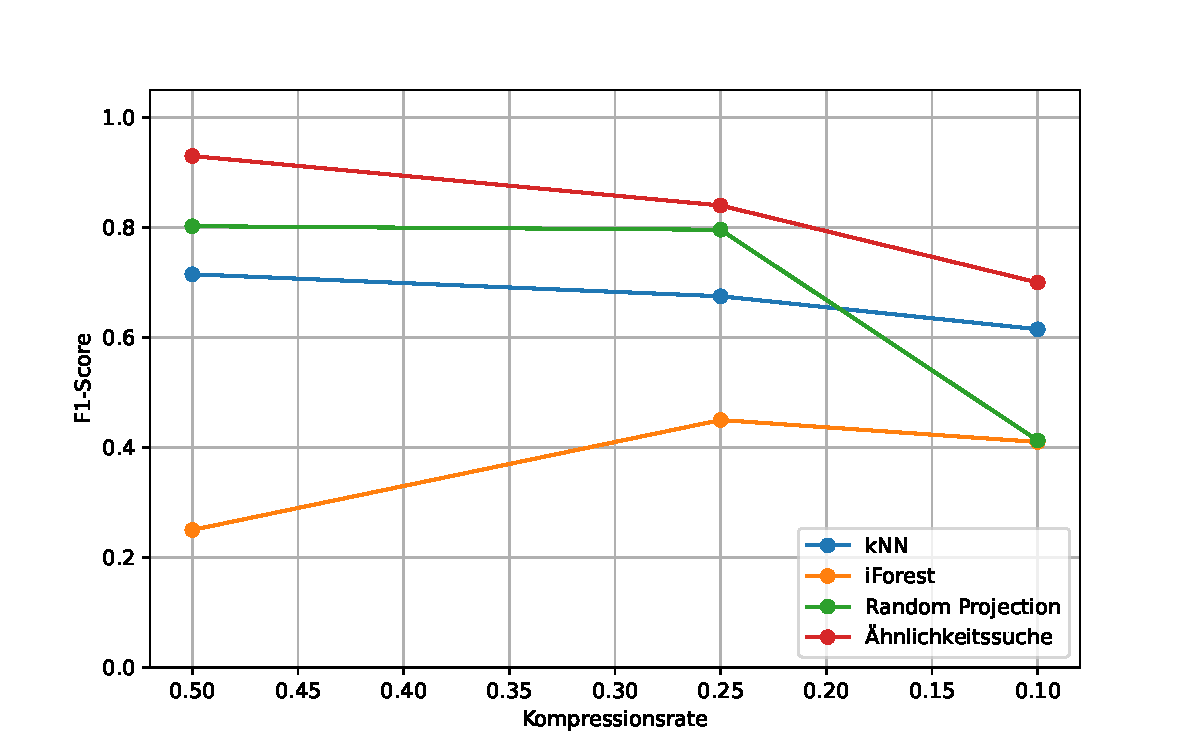
\includegraphics[width=0.49\textwidth]{Graphics/F1WaveletECG.pdf}\label{subfig:f1waveletecg}}
  \caption{F1"=Maße der Analyseverfahren bei Wavelet"=Kompression}
  \label{fig:f1WaveletMaße}
\end{figure}

\renewcommand{\tabledata}[4]{\phantom{0,000}\llap{#1} & \phantom{0,000}\llap{#2} & \phantom{0,000}\llap{#3} & \phantom{0,000}\llap{#4}\\}
% Linear Laufzeit
\begin{table}[h]
 \centering
 \begin{tabular}{lc|cccc}
  \toprule
  \multicolumn{1}{c}{\bfseries Daten} & \boldmath $\rho$ & \bfseries knn & \bfseries iForest & \bfseries Random P. & \bfseries Ähnl.suche \\ 
  \midrule
   \multirow{3}{*}{Wetterdaten} & 0,50 & \tabledata{0,081}{0,592}{0,168}{0,152}
   & 0,25 & \tabledata{0,065}{0,543}{0,094}{0,077}
   & 0,10 & \tabledata{0,066}{0,524}{0,060}{0,037}
   \midrule
   \multirow{3}{*}{NVIDIA-Aktie} & 0,50 & \tabledata{0,074}{0,971}{0,709}{0,488}
   & 0,25 & \tabledata{0,057}{0,641}{0,629}{0,352}
   & 0,10 & \tabledata{0,029}{0,641}{0,543}{0,236}
   \midrule
   \multirow{3}{*}{ECG5000} & 0,50 & \tabledata{0,138}{0,847}{0,417}{0,352}
   & 0,25 & \tabledata{0,107}{0,806}{0,294}{0,200}
   & 0,10 & \tabledata{0,117}{0,578}{0,234}{0,114}
  \bottomrule
 \end{tabular}
 \caption{Reduktion der Laufzeiten bei Linearer Kompression}
 \label{tbl:laufzeitlin}
\end{table}

% Poly Laufzeit
\begin{table}[h]
 \centering
 \begin{tabular}{lc|cccc}
  \toprule
  \multicolumn{1}{c}{\bfseries Daten} & \boldmath $\rho$ & \bfseries knn & \bfseries iForest & \bfseries Random P. & \bfseries Ähnl.suche \\ 
  \midrule
   \multirow{3}{*}{Wetterdaten} & 0,50 & \tabledata{0,073}{0,588}{0,161}{0,145}
   & 0,25 & \tabledata{0,058}{0,541}{0,091}{0,074}
   & 0,10 & \tabledata{0,056}{0,521}{0,058}{0,033}
   \midrule
   \multirow{3}{*}{NVIDIA-Aktie} & 0,50 & \tabledata{0,070}{0,971}{0,746}{0,513}
   & 0,25 & \tabledata{0,051}{0,641}{0,641}{0,351}
   & 0,10 & \tabledata{0,025}{0,637}{0,543}{0,227}
   \midrule
   \multirow{3}{*}{ECG5000} & 0,50 & \tabledata{0,138}{0,840}{0,418}{0,352}
   & 0,25 & \tabledata{0,067}{0,806}{0,294}{0,202}
   & 0,10 & \tabledata{0,078}{0,578}{0,232}{0,111}
  \bottomrule
 \end{tabular}
 \caption{Reduktion der Laufzeiten bei polynomieller Kompression}
 \label{tbl:laufzeitpol}
\end{table}

% Fourier Laufzeit
\begin{table}[h]
 \centering
 \begin{tabular}{lc|cccc}
  \toprule
  \multicolumn{1}{c}{\bfseries Daten} & \boldmath $\rho$ & \bfseries knn & \bfseries iForest & \bfseries Random P. & \bfseries Ähnl.suche \\ 
  \midrule
   \multirow{3}{*}{Wetterdaten} & 0,50 & \tabledata{0,130}{0,680}{0,339}{0,321}
   & 0,25 & \tabledata{0,080}{0,588}{0,176}{0,157}
   & 0,10 & \tabledata{0,088}{0,556}{0,127}{0,110}
   \midrule
   \multirow{3}{*}{NVIDIA-Aktie} & 0,50 & \tabledata{0,067}{0,980}{0,758}{0,562}
   & 0,25 & \tabledata{0,083}{0,971}{0,763}{0,546}
   & 0,10 & \tabledata{0,053}{0,971}{0,758}{0,513}
   \midrule
   \multirow{3}{*}{ECG5000} & 0,50 & \tabledata{0,183}{0,901}{0,592}{0,541}
   & 0,25 & \tabledata{0,098}{0,855}{0,498}{0,446}
   & 0,10 & \tabledata{0,186}{0,833}{0,288}{0,181}
  \bottomrule
 \end{tabular}
 \caption{Reduktion der Laufzeiten bei Fourier"=Kompression}
 \label{tbl:laufzeitfour}
\end{table}

% Wavelet Laufzeit
\begin{table}[h]
 \centering
 \begin{tabular}{lc|cccc}
  \toprule
  \multicolumn{1}{c}{\bfseries Daten} & \boldmath $\rho$ & \bfseries knn & \bfseries iForest & \bfseries Random P. & \bfseries Ähnl.suche \\ 
  \midrule
   \multirow{3}{*}{Wetterdaten} & 0,50 & \tabledata{0,070}{0,585}{0,158}{0,142}
   & 0,25 & \tabledata{0,051}{0,546}{0,098}{0,082}
   & 0,10 & \tabledata{0,051}{0,521}{0,054}{0,028}
   \midrule
   \multirow{3}{*}{NVIDIA-Aktie} & 0,50 & \tabledata{0,070}{0,971}{0,758}{0,518}
   & 0,25 & \tabledata{0,055}{0,637}{0,641}{0,368}
   & 0,10 & \tabledata{0,026}{0,637}{0,543}{0,228}
   \midrule
   \multirow{3}{*}{ECG5000} & 0,50 & \tabledata{0,133}{0,847}{0,391}{0,321}
   & 0,25 & \tabledata{0,060}{0,806}{0,283}{0,185}
   & 0,10 & \tabledata{0,126}{0,578}{0,238}{0,118}
  \bottomrule
 \end{tabular}
 \caption{Reduktion der Laufzeiten bei Wavelet"=Kompression}
 \label{tbl:laufzeitwav}
\end{table}

\begin{figure}[bth]
  \subfloat[ECG5000 - Linear - Random P. - 0,50]{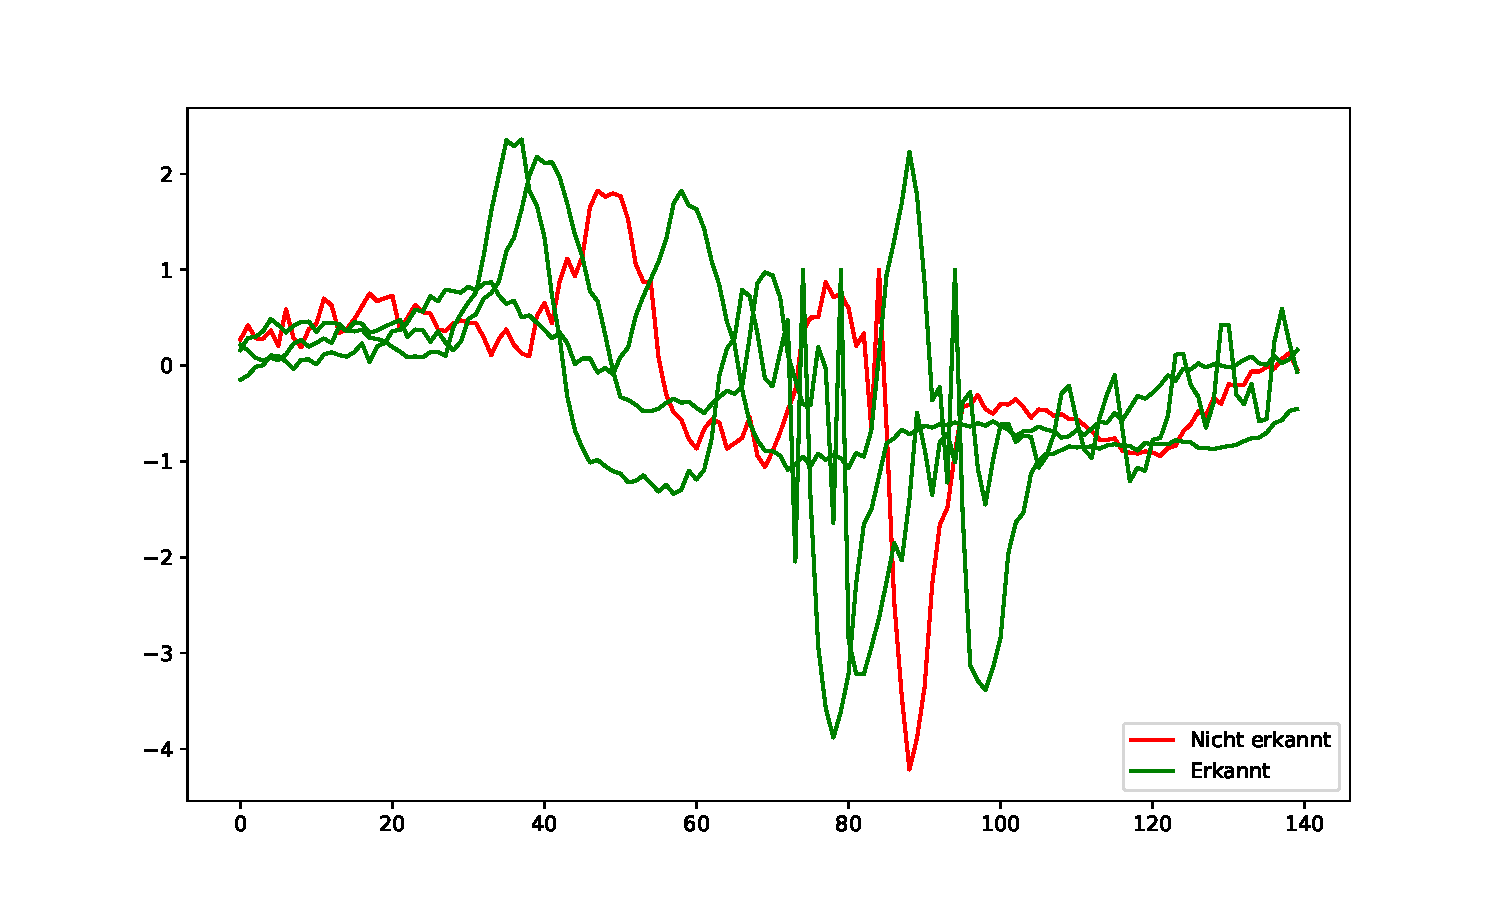
\includegraphics[width=0.49\textwidth]{Graphics/ausreisserECGLinRandom2.pdf}\label{subfig:abbone}}\hfill
  \subfloat[ECG5000 - Wavelet - Ähnl.suche - 0,10]{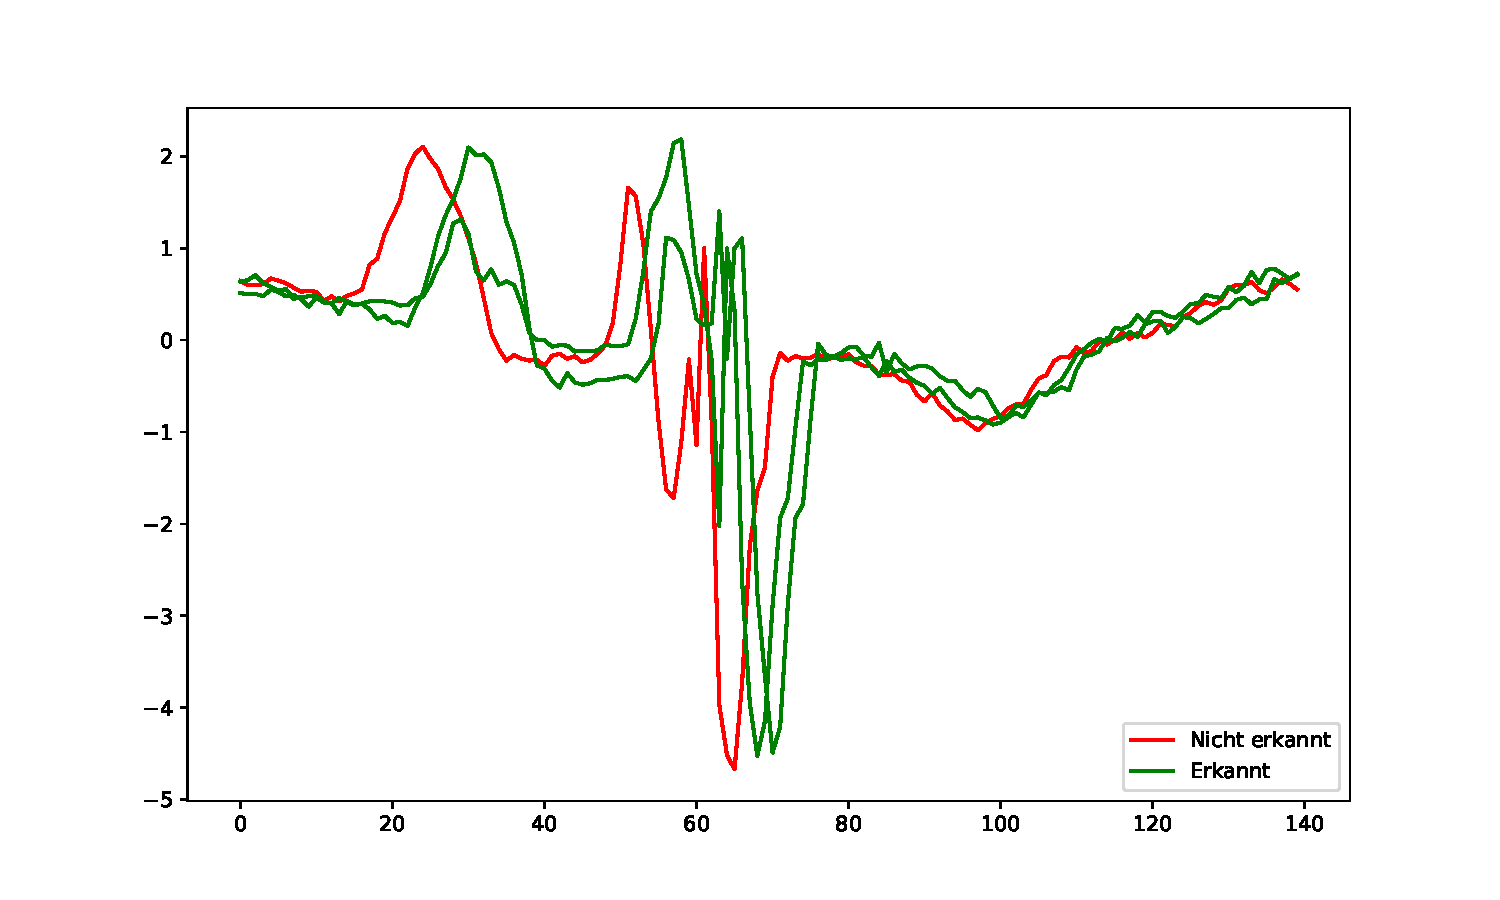
\includegraphics[width=0.49\textwidth]{Graphics/ausreisserECGWaveSimil10.pdf}\label{subfig:abbtwo}}\hfill
  \subfloat[NVIDIA - Wavelet - Random P. - 0,50]{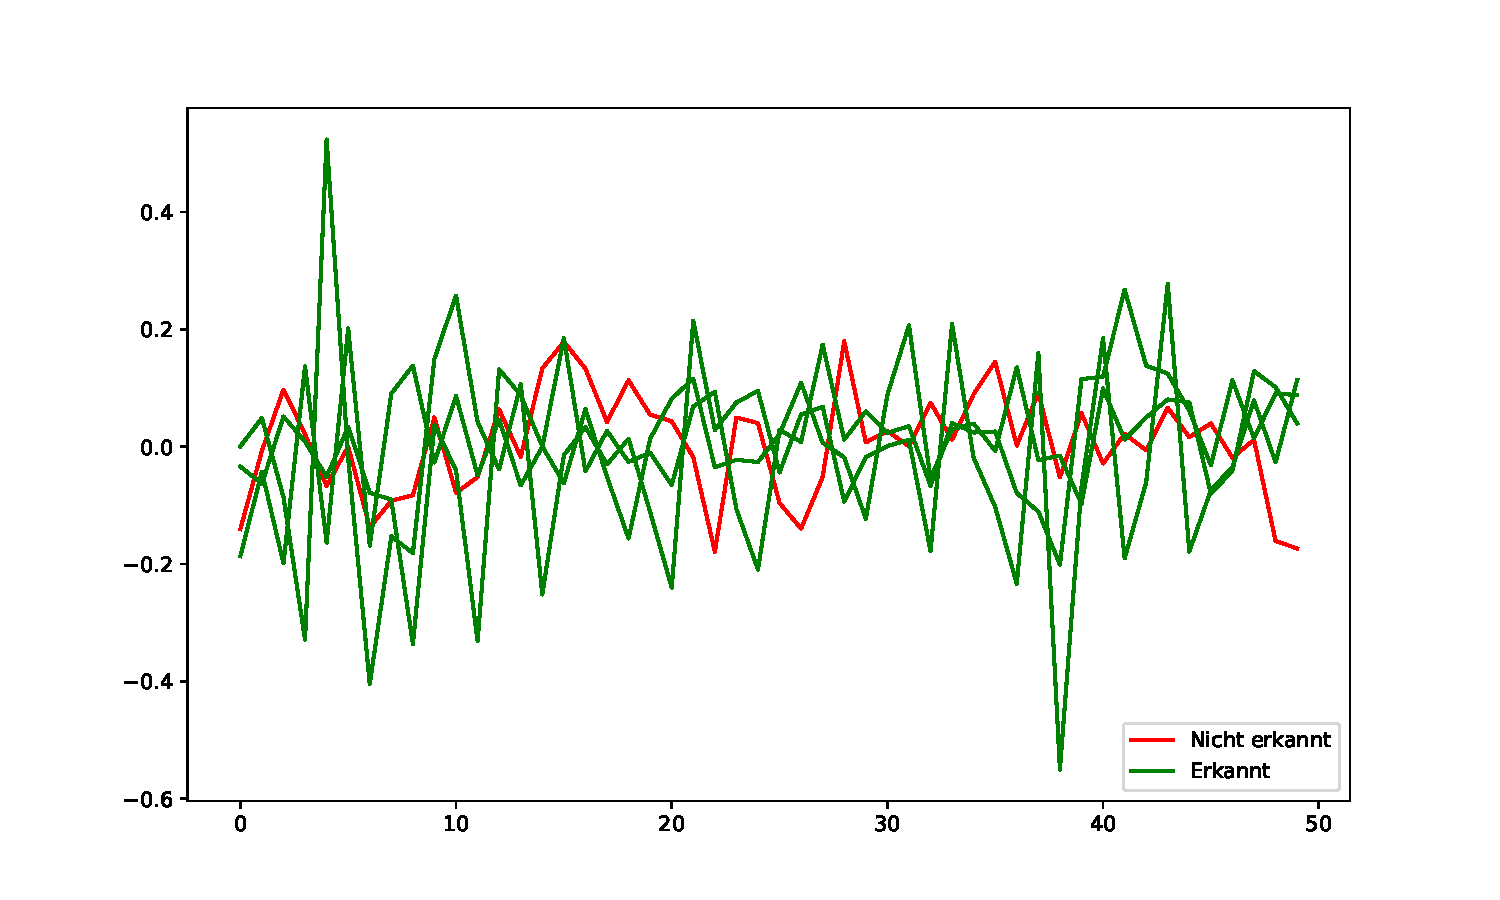
\includegraphics[width=0.49\textwidth]{Graphics/ausreisserNvidiaWaveletRandom2.pdf}\label{subfig:abbthree}}\hfill
  \subfloat[NVIDIA - Fourier - iForest - 0,25]{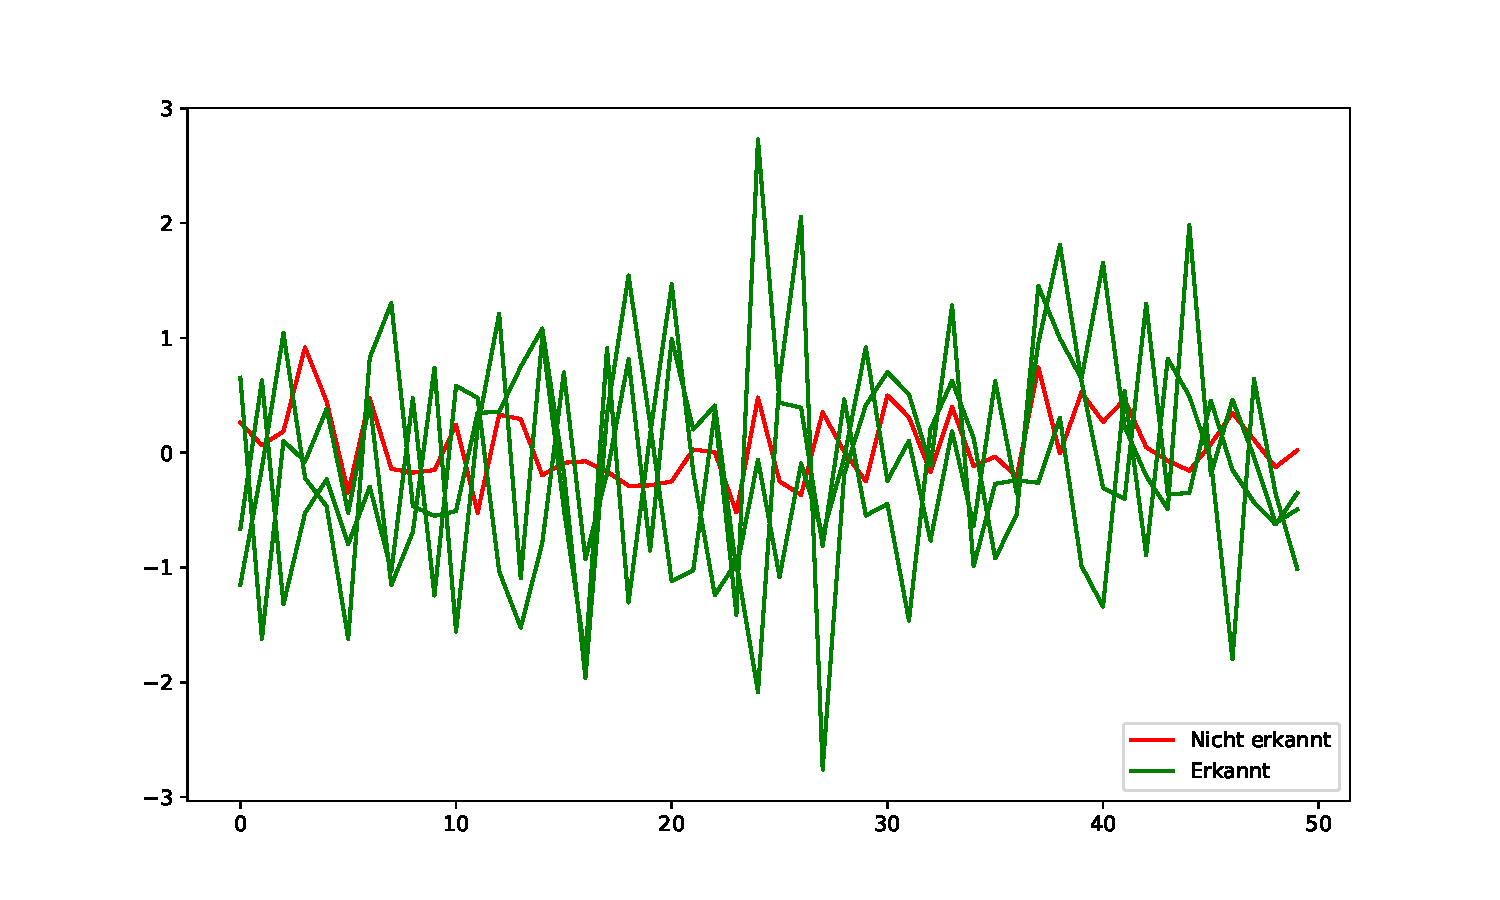
\includegraphics[width=0.49\textwidth]{Graphics/ausreisserNvidiaFourieriForest4.pdf}\label{subfig:abbfour}}\hfill
  \subfloat[Wetterdaten - Wavelet - knn - 0,50]{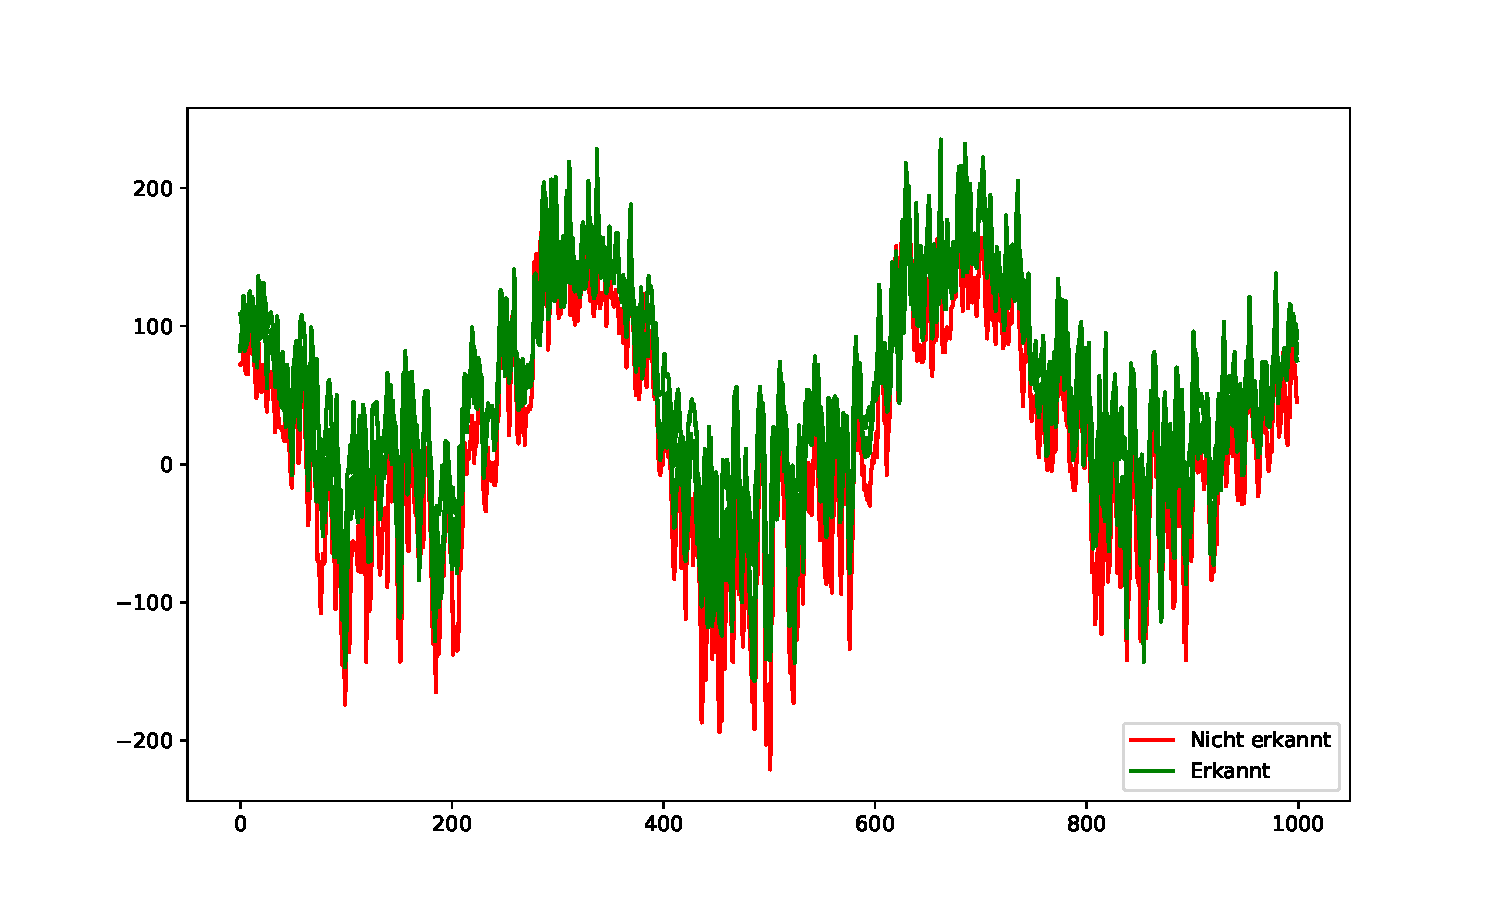
\includegraphics[width=0.49\textwidth]{Graphics/ausreisserWetterWaveletknn2.pdf}\label{subfig:abbfive}}\hfill
  \subfloat[Wetterdaten - Polynomiell - iForest - 0,25]{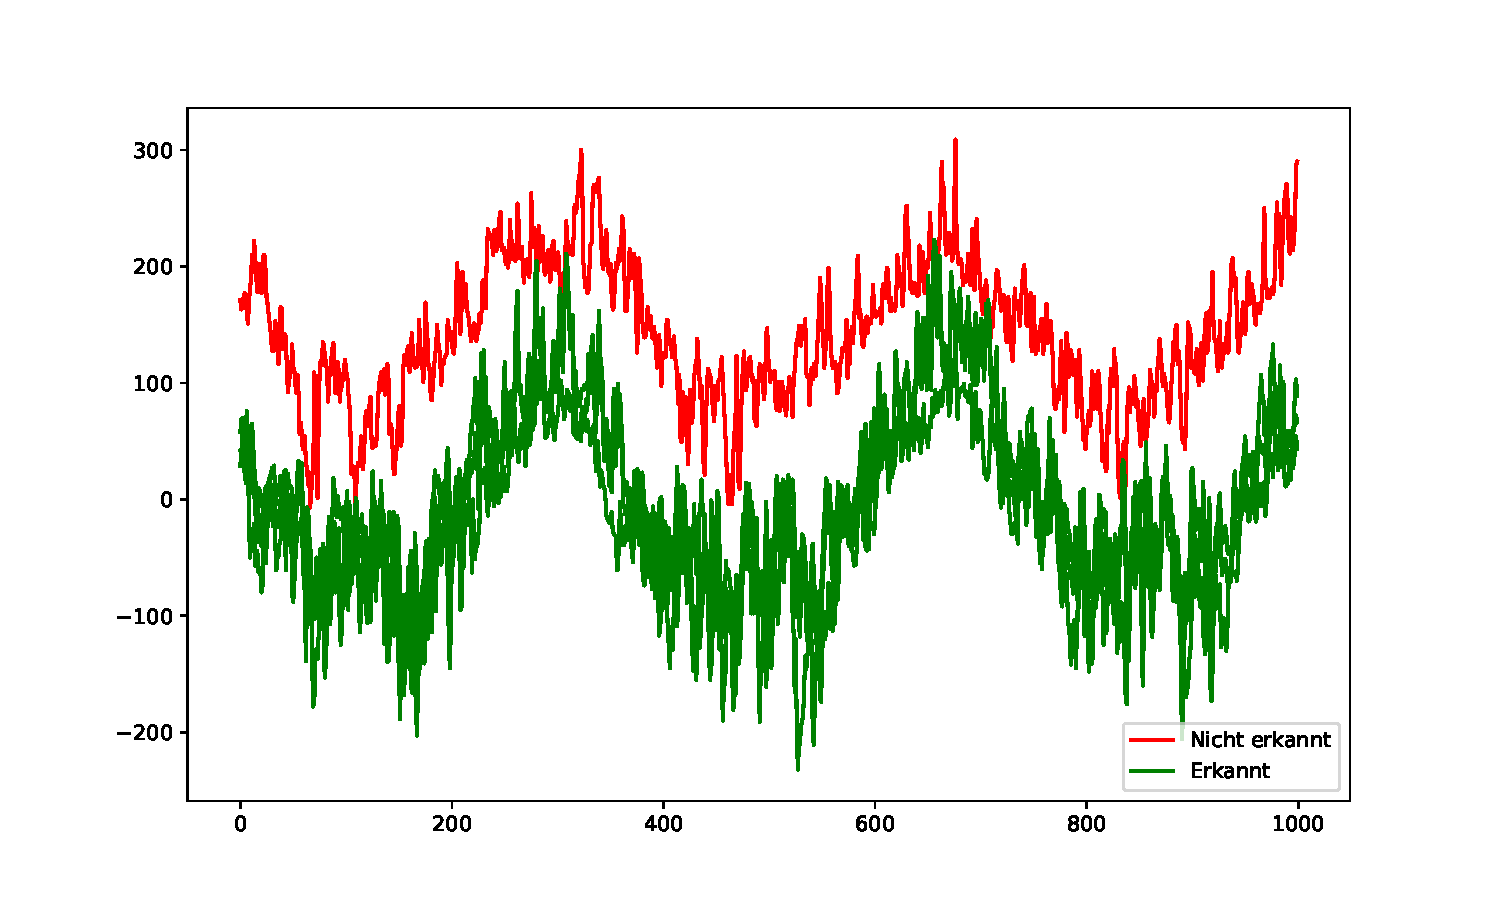
\includegraphics[width=0.49\textwidth]{Graphics/ausreisserWetterPolyiForest4.pdf}\label{subfig:abbsix}}
  
  \caption{Beispiele von Ausreißern die nach der Kompression nicht mehr erkannt wurden}
  \label{fig:alle}
\end{figure}